\begin{figure}[h!]
\centering
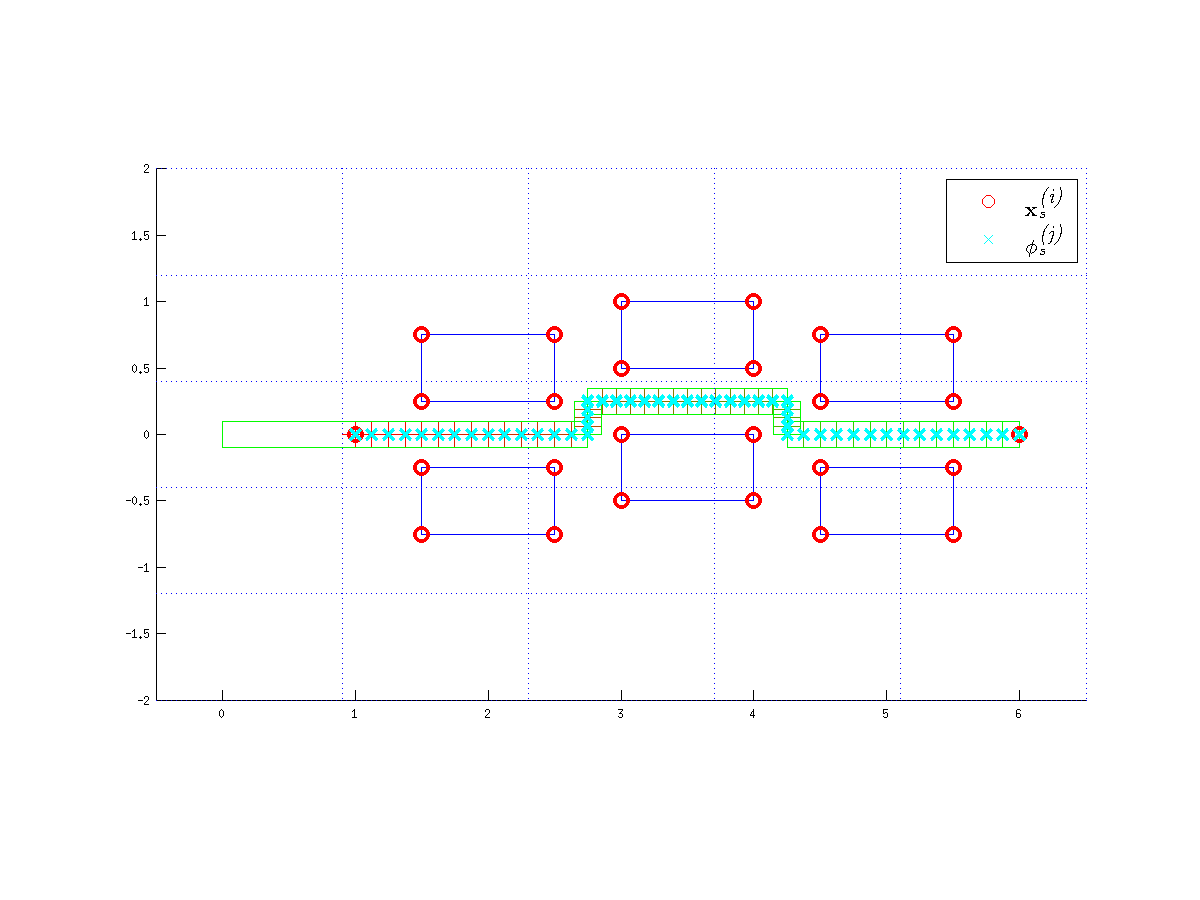
\includegraphics[width=0.5\textwidth]{scopey_demo}
\vspace{-1cm}
\caption{Demonstration trajectory for robot with telescoping links. The blue rectangles are the obstacles, the red points indicate the scene correspondence points, and the green outline and red line trace the trajectory of the robot.}
\label{fig:scopey_demo}
\end{figure}

\begin{figure}
\centering
\begin{subfigure}[b]{.32\textwidth}
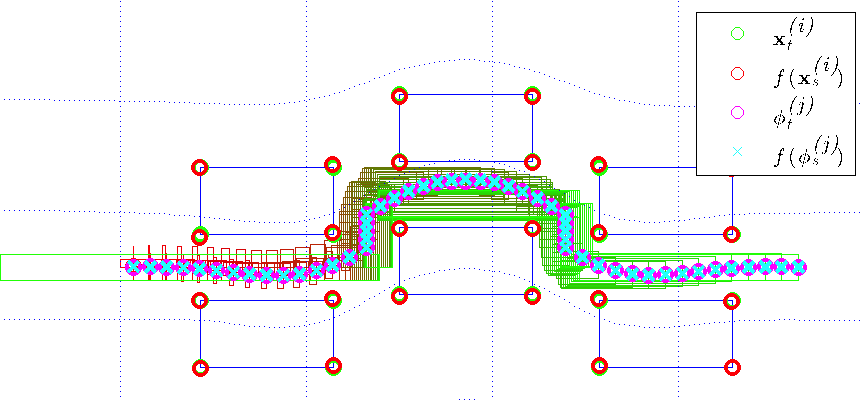
\includegraphics[width=\textwidth]{twostep_offset0-30_cropped}
\caption*{two-step with offset 0.3}
\end{subfigure}
\begin{subfigure}[b]{.32\textwidth}
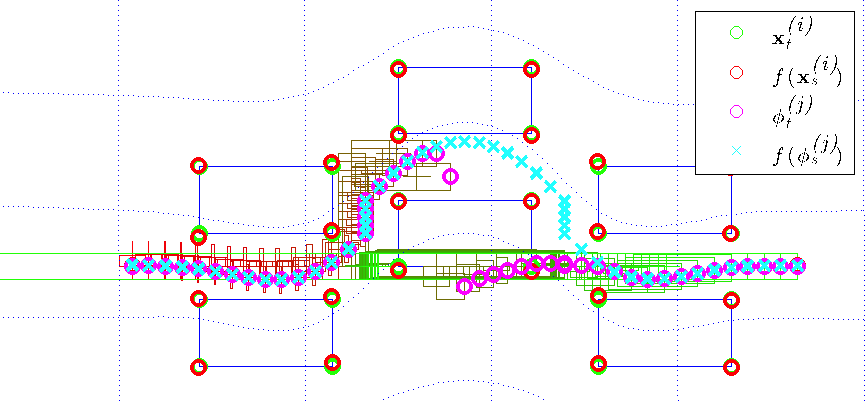
\includegraphics[width=\textwidth]{twostep_offset0-50_cropped}
\caption*{two-step with offset 0.5}
\end{subfigure}
\begin{subfigure}[b]{.32\textwidth}
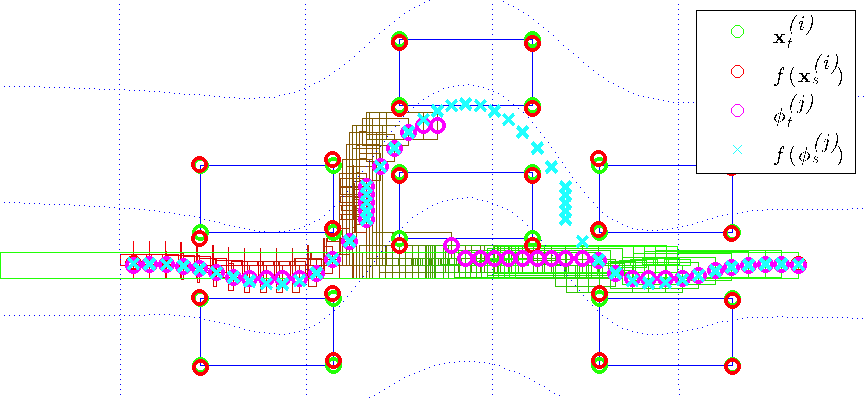
\includegraphics[width=\textwidth]{twostep_offset0-70_cropped}
\caption*{two-step with offset 0.7}
\end{subfigure}\\
\begin{subfigure}[b]{.32\textwidth}
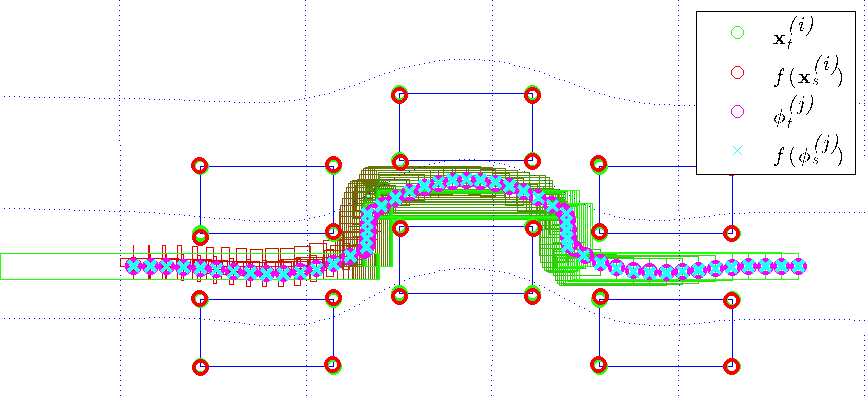
\includegraphics[width=\textwidth]{joint_offset0-30_cropped}
\caption*{unified with offset 0.3}
\end{subfigure}
\begin{subfigure}[b]{.32\textwidth}
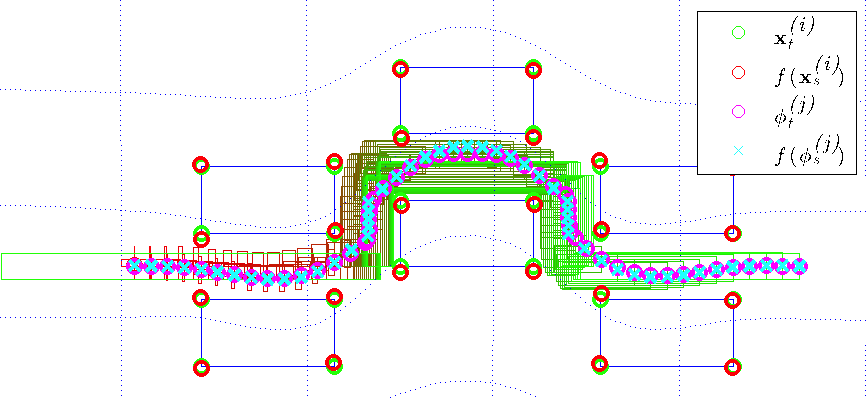
\includegraphics[width=\textwidth]{joint_offset0-50_cropped}
\caption*{unified with offset 0.5}
\end{subfigure}
\begin{subfigure}[b]{.32\textwidth}
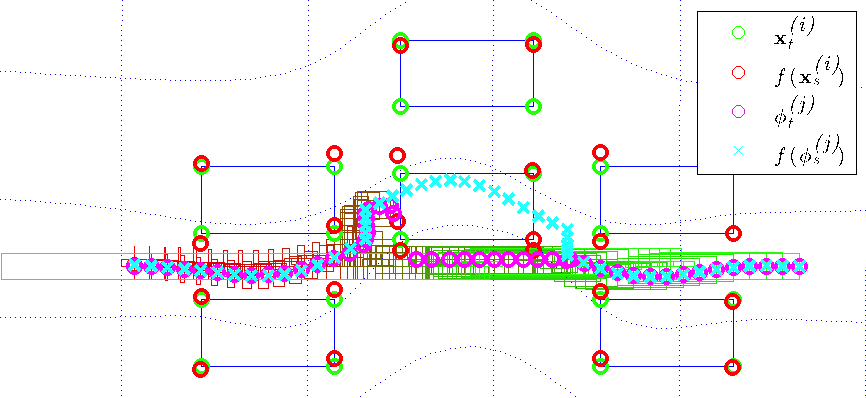
\includegraphics[width=\textwidth]{joint_offset0-70_cropped}
\caption*{unified with offset 0.7}
\end{subfigure}\\
\caption{The warped blue grid shows the registration from the demonstration scene to the new scene, in which the two middle obstacles are shifted slightly upwards. For an offset of 0.5, two-step optimization does not find a feasible trajectory whereas unified optimization is able to find one.}
\label{fig:scopey_results}
\end{figure}

We also applied our formulation to a robot with five telescoping links (three horizontal links interconnected by two vertical links). In the demonstration (Figure~\ref{fig:scopey_demo}), we specify a trajectory for the robot to navigate through a tunnel formed by three pairs of rectangular obstacles. In the new scenes, the middle pair of obstacles is shifted upwards by varying amounts (Figure~\ref{fig:scopey_results}). For small upward shifts (e.g. 0.3), the warping functions and proposed trajectories found by the two-step optimization and our unified optimization are essentially identical. However, when the upward shift is increased to 0.5, the two-step optimization is unable to find a feasible trajectory, whereas our unified optimization approach finds a feasible trajectory by finding a warping function that warps the scene more sharply upwards near the middle pair of obstacles.

When the new scene differs significantly from that of the demonstration (e.g. an upward shift of 0.7), both optimization approaches fail to find the desired feasible trajectory that passes between all three pairs of obstacles. In the unified optimization the tradeoff between matching correspondence points and finding a feasible trajectory is clear, since the warping function no longer matches the correspondence points on the corners of the middle pair of obstacles, in order to make the warped original trajectory closer to a feasible one. These experimental results on the telescoping robot show that in certain new scenarios, using unified optimization allows for greater generalization of demonstrations.
